%\documentclass[prb,preprint]{revtex4} 
\documentclass[twocolumn,preprintnumbers,amsmath,amssymb,aps,prx]{revtex4}
% The line above defines the type of LaTeX document.
% Note that AJP uses the same style as Phys. Rev. B (prb).

% The % character begins a comment, which continues to the end of the line.
\usepackage{amsmath}  % needed for \tfrac, \bmatrix, etc.
\usepackage{amsfonts} % needed for bold Greek, Fraktur, and blackboard bold
\usepackage{graphicx} % needed for figures
\usepackage{pythontex}

\begin{document}

% Be sure to use the \title, \author, \affiliation, and \abstract macros
% to format your title page.  Don't use lower-level macros to  manually
% adjust the fonts and centering.

\title{Molecular dynamics simulation of synchronization in driven particles}
% In a long title you can use \\ to force a line break at a certain location.

\author{Tiare Guerrero}
\email{guer9330@pacificu.edu} % optional
%\altaffiliation[permanent address: ]{101 Main Street, 
%  Anytown, USA} % optional second address
% If there were a second author at the same address, we would put another 
% \author{} statement here.  Don't combine multiple authors in a single
% \author statement.
%\affiliation{Department of Physics, Pacific University, Forest Grove, OR 97116}
% Please provide a full mailing address here.

\author{Danielle McDermott}
\email{mcdermott@pacific.edu}
\affiliation{Department of Physics, Pacific University, Forest Grove, OR 97116}

% See the REVTeX documentation for more examples of author and affiliation lists.
\date{\today}

\begin{abstract}
  Synchronization
  plays a key role in many physical processes.
  %Simplified models
  %such as 
  %What problem did you study and why is it important?
  Particles
  %confined to a narrow channel 
  driven
  across a washboard potential energy landscape
  move in 
  synchronized patterns,
  as observed in 
  experiments %al systems 
  of %interest to condensed matter physics %including 
  magnetically driven colloidal particles
  confined by light-fields.
  %exhibit a variety of synchronization effects.
  %in
  %  Numerical model
  We discuss a simple
  numerical model that
  %exhibits
  provides insight
  to synchronization behavior
  %and
  %atoms on surfaces.
  %voltage driven superconducting vortices
  %confined in a Josephson junction,
  %and ac and dc driven
  %charge and spin density waves.
  %We present the basics
  using
  molecular dynamics simulations
  for particles moving through
  a viscous liquid.
  %
  %applied to single and multiple particle systems.
  %so we model the dynamics of each particle
  %with 
  %overdamped equations of motion.
  Our results show a variety of synchronization effects 
  in single and multi-particle systems, 
  %and detect synchronization using
  %measurements of
  which we characterize with
  plots of 
  particle velocity as a function of applied driving force,
  and phase diagrams of position versus velocity.
  %We demonstrate how to 
  %visualize
  %the system with
  %numerical representations of the landscape
  %and
  %animations of the particle motion.
  %We include sample code
  %and exercises for students
  %with 
  %opportunities
  %to reproduce our results and propose
  %new numerical experiments.
  %With only a few particles in two-dimensions,
  %the simulation runs quickly,
  %making this an appropriate model for undergraduates to explore.  
\end{abstract}
% AJP requires an abstract for all regular article submissions.
% Abstracts are optional for submissions to the "Notes and Discussions" section.

\maketitle % title page is now complete

\section{Introduction} %
%
%Outline
%------------------------------------------------------------------
%synchronization = widest audience possible
Synchronization is a universal phenomena
in which individual oscillators adjust frequency due
to external stimulus \cite{Pikovsky2003}.
Many everyday systems
exhibit in-phase oscillations of components 
such as the
flickering patterns of
candle flames coupled by temperature fluctuations \cite{Okamoto2016},
vibrations of singing wineglasses \cite{Arane2009}, 
and metronomes coupled through a supporting platform \cite{Jia2015}.
Biological systems benefit from cooperative
synchronization -- %such as 
birds coordinate wing flaps
to optimize energy use during flight \cite{Portugal2014},
frogs alternate croaking patterns \cite{Aihara2014},
humans clap in time with music \cite{Tranchant2016}
and 
at a cellular level, 
neurons simultaneously fire in cardiac muscle \cite{MartinHall1999}
and brain tissue \cite{Singer1999}.
External forcing can cause or regulate 
synchronization. % is often achieved via external forcing
%such as when
%single particle oscillators
For instance,
an electrical pacemaker %(an electrical generator)
pulses to regulate a heart beat,
and 
a flashing light can modify the
pattern of flashing fireflies .% \cite{Agrawal2013}.

%Christiaan Huygens 
%[has been adapted into many useful technologies...]
A particular form of 
synchronization is phase-locking or mode-locking,
which first appeared in the scientific literature
with 
Huygens' 1665 experiments on
the 
motions of two wall-mounted pendulum clocks.
Huygens demonstrated the tendency of
the pendula 
%two periodic oscillators in close proximity
to swing in time %, i.e. to synchronize,
due to interactions through the wall,  
no matter the original phase of the clocks \cite{Bennett2002}.
%phase locking
Dynamical systems %with multiple frequencies
exhibit phase-locking 
when oscillators with different rhythms adjust %couple
to a frequency ratio or mode 
of an integer number \cite{Bak1986}.
%Dynamical mode locking
%The phenomena
Synchronization 
is often studied with simple computational models
and can be visualized 
with phase
plots or Lissajous figures.
In phase space 
a mode-locked system is confined to 
a closed loop in a 
parametric space showing the relationship between two periodic functions
with patterns determined by the mode, % frequency ratio,
first reported in 1857 \cite{Lissajous1857}
and easily generated with a computer code 
or oscilloscope \cite{Tong1997}. 
%with a frequency generator,
%where two combined frequencies at perpendicular orientations
%({\it As we will demonstrate in phase plots in Figs. X, Y, Z})
It should be noted that oscillation phase and phase space
  refer to different uses of the word ``phase.''  Oscillation
  phase $\phi_0$ is the constant portion of the argument in a periodic function
  $\sin{(\omega t + \phi_0)}$ while phase space refers
  to plots of velocity versus position (such as $v_y$ vs. $y$)
  that are used to characterize oscillating systems.
 

%Given the prevalence of synchronization,
%it is the subject of many computational models.
Here we perform numerical studies 
on the synchronized dynamics
of confined particles driven over
a washboard shaped potential energy landscape.
%Numerical studies %of harmonic systems
%can yield insights
%to the mechanics of naturally oscillating systems.
We chose this model for its
relevance to condensed matter systems
and ease of simulation.
%---------------------------------------------------------------
%kinks and nanofriction
%-----------------------------------------------------------------
%transition from synchronized to chaotic
%describe types of physical systems - particle types
%%In this work,
%we perform 
%numerical simulations of confined, driven particles
%to model a variety of physical phenomena.
%-----------------------------------------------------------------------
%paper outline
%In the following paper
In Section~\ref{sec:colloids} we describe colloid particles,
an relevent
experimental analog of our simulations.
We describe
our molecular dynamics model for a single particle in Section~\ref{sec:MD}.
%In this section, we restrict our discussion to a single particle,
%and include additional information
%for multiple particles in Section~\ref{sec:sync}.
%including various  and confining environments.
We summarize
our results 
%in Section~\ref{sec:results} 
including synchronized motion of a single confined particle
driven across a periodic landscape in 
Section~\ref{sec:one}.
In Section~\ref{sec:sync}
we 
extend the model to include multiple particles,
and show how confined 
interacting particles respond to the same applied driving force.
%including stationary propagation of high density kinks
%in Sec.~\ref{sec:kink}.
%We include code to simulate
%and visualize the landscape and dynamics in this section
%and supplementary material.
%we
%demonstrate how uniform environments and applied forces
%and create synchronized flow patterns.
%We present these results using standard tools of non-linear oscillators
%such phase diagrams of velocity versus position.
%PHASE DIAGRAMS SHOWING COUPLING, OR QUASI-PERIODIC COUPLING
%INDICATE COOPERATIVE MOTION IN THE Q1D SUBSTRATE
%In Section~\ref{sec:quasiperiod},
%we show how an aperiodic landscape modifies the particle dynamics.
%Finally we explore the transition to chaotic dynamics in 
%Section~\ref{sec:chaos}
%and conclude 
In Section~\ref{sec:conclusion}
we describe how our work with colloids applies more broadly
to many physical systems
such as dusty plasmas, superconducting vortices and Josephson junctions.
We conclude with
exercises for interested students 
in Section~\ref{sec:problems}.


\section{Colloidal Models}
\label{sec:colloids}

Complex dynamics can be studied with
colloid particles with experiments and simulation.
In typical experiments colloids are spheres of 
plastic suspended in
highly de-ionized water or silica in suspended in organic solvent.
%experimental - colloids specifically
Because 
the spheres are a few microns in size
and move at rates of microns per second,
the position of a particle %is large and slow enough to
can be imaged as a function of time 
with a traditional optical camera.
%due to the large size and slow speed of the particles.
Individual colloids exhibit 
Brownian motion,
where particles change direction %in a seemingly random fashion
due to 
collisions 
with unseen particles comprising the suspending fluid \cite{}.
%[elaborate - move to associated problems?].

Light is a
tool for manipulating the colloidal environment.
A single laser beam can be used to create an optical trap,
which uses 
photon radiation pressure to
control colloid motions \cite{Ashkin1997}.
A circular optical trap is designed so the center is
a local energy minimum where 
a colloid in the beam center is subject to a
uniform distribution of photon bombardment. %, making 
Colloids at a trap edge
experience a net force
due to the uneven 
distribution of photon collisions on its surface.
Depending on the shape of the trap and location of the particle in the trap,
the radiation pressure either pushes colloids toward the local minima
or ejects it from the trap.
A single optically trapped colloid executing Brownian motion
is a useful probe of microscopic forces,
and has been studied in detail in Ref.~\cite{Volpe2013}.


Experiments of colloid particles confined
in optical traps arrays or patterns 
subject to external driving forces 
have
been used to examine the microscopic dynamics
of individual particles during mode-locking \cite{Juniper2015}.
This produced step-by-step diagrams
of particle dynamics that cannot be 
imaged in electronic systems such as Josephson junctions.
%Recent work with atomic systems such as Bose-Einstein condensates \cite{Zhang2020}
Thus the study of
mode-locking is a useful problem
of complex quantum mechanical systems.

%external forces
%The
%dynamics of particles subject to 
%an applied external force apply to many physical systems.
%For instance the flow of charges in a conductor,
%or cells responding to a chemical gradient.
%The external force 
%increases the diversity of dynamical behaviors,
%and can cause particles to flow in
%a variety of non-linear complex patterns
%that may be 
%synchronized.
%Disordered chaotic dynamics are also possible,
%where irregular, unpredictable time evolution of
%nonlinear systems occurs in mechanical oscillators \cite{chaos}.
%-------------------------------------------------------------

Numerical modeling of colloids can provide mechanistic insight
that can be difficult to achieve in experimental conditions
where Brownian motion and other sources of noise dominate.



%Here we model the microscopic dynamics of phase locking in a colloidal model syestem using molecular dynamics (MD).

\section{Molecular Dynamics Simulation}
\label{sec:MD}

We use a classical model for 
studying the dynamics of $N$ interacting particles,
using the net force on each particle to calculate
its trajectory.
Particles are confined in a two-dimensional (2D) 
simulation of area $A = L \times L$ where $L=36.5 a_0$
where $a_0$ is a dimensionless unit of length.
An individual particle $i$ has
position $\vec{r}_i = x_i \hat{x} + y_i \hat{y}$
and velocity $\vec{v}_i = d\vec{r}_i/dt$.
The edges of the system are treated with
periodic boundary conditions
such that a particle leaving the edge of the system is mapped
back to a position within the simulation boundaries 
by the transformation $x_i+L \rightarrow x_i$ and $y_i+L \rightarrow y_i$.
%and particles interact across PBC.
We show a schematic of the system in Fig.~\ref{fig:landscape0}(a).

We confine the particles using a position dependent 
potential energy function, called a landscape or substrate.
 %The landscape potential energy $U(\vec{r})$ is static 
 %with fixed minima and maxima
 %that are periodic or quasi-periodic,
 %as described in Sec.~\ref{sec:results}.
% 
The landscape is modulated in the y-direction
with the periodic function 
%% %that used in Sec.~\ref{sec:one}
% where 
 \begin{equation}
   U(y) = U_0 \cos{(N_p \pi y / L)}
     \label{eq:ysubstrate}
\end{equation}
 where $N_p$ are the number of periods,
 % $L$ is the period length,
 and $U_0$ is an adjustable parameter
 to set the depth of the minima
 with simulation units of energy $E_0 = 1$. 
 %We define the substrate strength to be
 %the maximum force the substrate can exert on a particle 
 %$A_p = 2\pi U_0/L$.
 %
 In experiment 
 complex environments can be
 engineered with light by %, typically made 
 using diffraction gratings to create a patterned
 potential energy landscape 
 with one or more laser beams \cite{}.
 %
 We plot this function in 
 Fig.~\ref{fig:landscape0}
 we use $N_p = 3$ to illustrate the features of
 Eq.~\ref{eq:ysubstrate}.
 In Fig.~\ref{fig:landscape0}(a) we show 
 the $x-y$ plane with a contour plot
 of the the 2D potential energy landscape,
 where 
 the maxima are colored red and the minima colored blue.
 The confining force on a particle $i$
 %arises from a potential function 
 %creating a landscape of potential minima and maxima
 %that modify the force on a particle as a function of position
 is calculated as 
 $\vec{F}^{l}_i(\vec{r}_i) = -\nabla U_l(\vec{r}_i)$.
 In Fig.~\ref{fig:landscape0}(b) we plot the function
 $U(y)$ to illustrate how the magnitude
 $\vec{F}^{l}_i$ is calculated from particle position $y_i$.  
 %in the $y-$direction.
 
\begin{center}
\begin{figure}[h!]
\centering
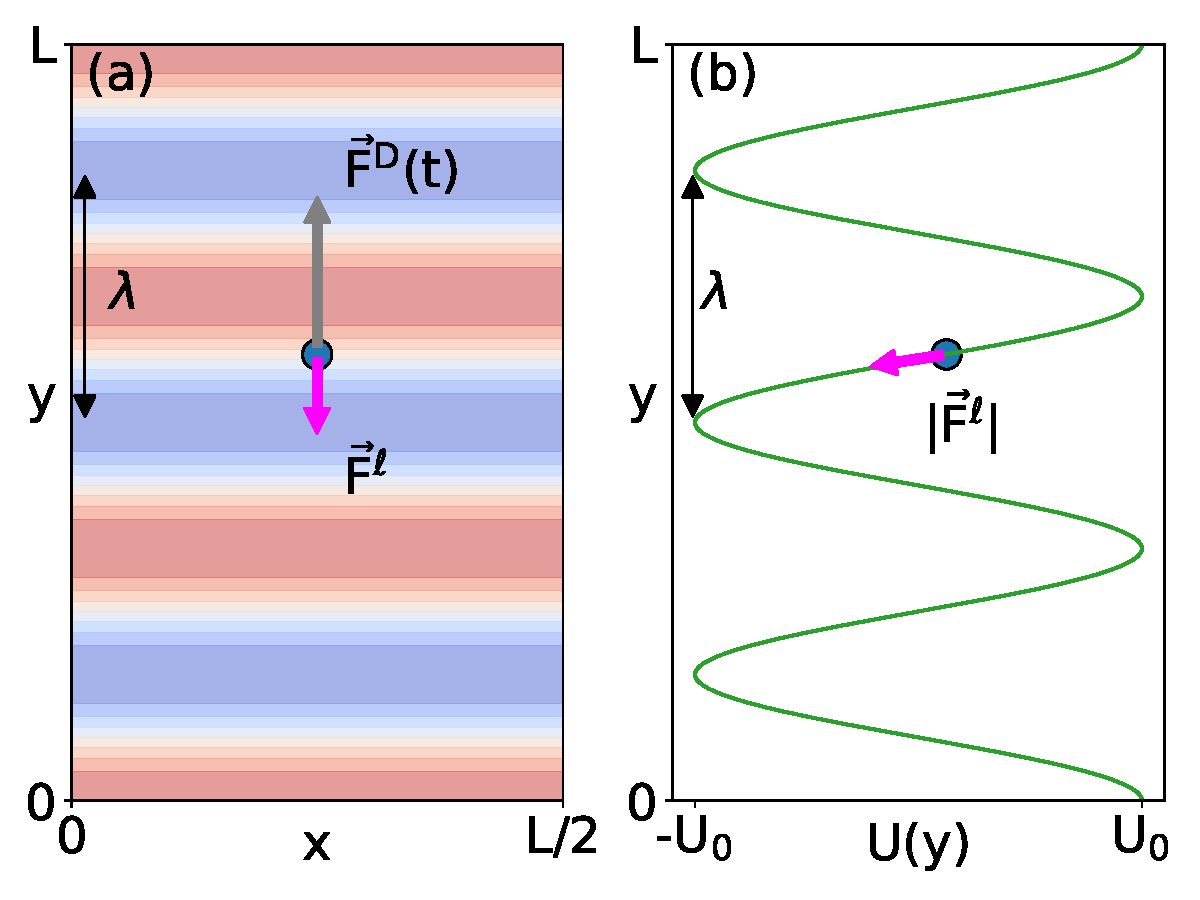
\includegraphics[width=\columnwidth]{landscape.pdf}
\caption{
  Schematic of the simulation
  of a single particle
  driven across a washboard potential
  energy landscape.
  The period of the landscape, $\lambda = L/N_p$ 
  where $N_p = 3$, is marked in red.
  The force due to the landscape %$\vec{F}^l$
  is calculated from the gradient of the potential
  energy 
  $\vec{F}^l = -\nabla U(\vec{r})$.
  (a) View of the $x-y$ plane. %of the simulation
  The time-dependent applied driving force $\vec{F}^d$
  is parallel to the y-axis.
  The landscape is shown with a contour plot,
  with maxima in the potential energy marked in red
  and minima marked in blue.
  A particle is shown in the region between minima and maxima
  subject to competing forces due to the landscape and applied driving force.
  (b) The potential energy function
  along the y-axis $U_l(y)$,
  The particle in (a) is shown at the same $y-$position,
  where the magnitude of force $\vec{F}^l$ is calculated as the slope of this function,
  directed along the $y-$direction in panel (a).
  }
\label{fig:landscape0}
\end{figure}
\end{center}

 
 Particles are subject an external time-dependent driving force
$\vec{F}_{D}(t)$
applied parallel to the y-direction.
We model this force as
\begin{equation}
  \vec{F}^{d}(t) = [F^{dc} + F^{ac} \sin(\omega t)] \hat{y},
    \label{eq:drive}
\end{equation}
with modifiable parameters including
a constant component $F^{dc}$,
and a time dependent component with amplitude $F^{ac}$
and frequency $\omega = 2 \pi f$.
%in the positive $y-$direction.
%but it may 
%be zero or negative depending the the parameters and time.
When $F^{dc}$ is non-zero,  
%In several simulations
we slowly increase 
$F^{dc}$ from zero
to avoid transient behavior
by ensuring the particle is subject to a smoothly varying force.
We illustrate the increase
of $F^{dc}$ in Fig.~\ref{fig:0}(a).

%because
The inertia of 
small particles is greatly reduced by interactions
with fluid particles \cite{Purcell1977}.
Our model 
colloids are overdamped
-- i.e. suspended in a continuous viscous fluid
that dissipates energy at a rate such 
that the particles do not accelerate.
%that greatly impedes their motions.
Energy dissipation from the fluid is modeled
with a frictional force on particle with velocity $\vec{v}_i$
%that removes energy from
%the particles,
%which we model as
$\vec{F}^{drag}_i = -\eta \vec{v}_i$
%proportional to the particle velocity 
with a friction coefficient $\eta$
proportional to the fluid viscosity.
We discuss friction models for
spheres moving through fluids in 
Section~\ref{sec:problems} Exercise~\ref{ex:reynolds}. %for more information
%We model the particle dynamics  with an overdamped equation of motion. Models with inertia set to zero are appropriate for moving through a high viscosity fluid
Newton's second law for an individual particle
%$m \vec{a}_i = \sum \vec{F}$
is simplified
by the assumption $\vec{a}_i$ is zero. % in the overdamped model.
%Newton's second law can be rearranged %for the velocity
%to
The overdamped equation of motion for an isolated particle is
%solved for velocity 
\begin{equation}
  \eta \vec{v}_i = \vec{F}^l_{i} + \vec{F}^{d}(t).
    \label{eq:motion}
\end{equation}
with  $\eta = 1$.  
%which we describe in more detail in Table~\ref{tab:1}
%and Exercise~\ref{ex:reynolds}.
In %Section~\ref{sec:problems}
Exercise~\ref{ex:n2l}
we invite the reader to confirm this result.

The equation of motion provides a direct calculation of the velocity
of an individual particle from its location $\vec{r}_i$ %in the simulation
and the simulation time.
The molecular dynamics simulation is controlled by a $for()$ loop
 which runs from an initial to maximum integer number of time steps $t_i$.
Each integer time step interval $t_{i+1}-t_i$
represents a simulation time interval of $\Delta t$ 
simulation units.  %as described in Table 1
At each time step
we evaluate the net force on each particle as a function of its position
$\vec{r}_i(t)$
and then integrate
the equation of motion to move particles
to an updated position
$\vec{r}_i(t+\Delta t)$.
%
Since the acceleration as zero,
the integration of the equation of motion
is performed via 
the Euler method 
\begin{equation}
  \vec{r}_i(t+\Delta t) = \vec{v}_i(t) \Delta t + \vec{r}_i(t)
    \label{eq:euler}
\end{equation}
for a small time step $\Delta t$.
In Section~\ref{sec:problems} Exercise~\ref{ex:euler}
we elaborate on
the numerical methods for 
solving differential equations,
and demonstrate how the Verlet method
simplifies to the Euler method when $\vec{a}=0$.
%
The units of the simulated variables are summarized in Table ~\ref{tab:1}.

\begin{table}[h!]
\centering
\caption{Simulation units.}
\begin{ruledtabular}
\begin{tabular}{c c p{5cm}}
Quantity & Unit \\
\hline
length &  $a_0 = 1$ \\
energy & $E_0 = 1$ \\
%electric potential & $V(r_{ij}) = E_0/r_{ij}$ \\
%energy & $E_0 = q^2{Z^*}^2/4\pi \epsilon \epsilon_0 a_0$ \\
%dimensionless interaction strength & $q$ \\
%effective colloidal charge & $Z^*$ \\
%solvent dielectric constant & $\epsilon \epsilon_0$\\
force & $F_0 = E_0 / a_0$\\
velocity &  $ a_0 / \tau $ \\
viscosity coefficient & $\eta = F_0 \tau / a_0 = 1 $\\
time &  $ \tau = \eta a_0 / F_0 $ \\

\end{tabular}
\end{ruledtabular}
\label{tab:1}
\end{table}

%\section{Results}
%\label{sec:results}
% We demonstrate how a single particle (Sec.~\ref{sec:one})
% and many particles
% move (Sec.~\ref{sec:sync})
% in response to this applied force in a variety of environments.
% In Sec.~\ref{sec:kink} we set $F^{dc}$
% to zero and track the motion
% of a high density area of a particle chain
% (i.e. kink dynamics).
 %The driving force does add energy into the system, and some of it is lost.
%
\section{Mode-locking of a single particle}
% In subsection headings, only the first word is capitalized.
\label{sec:one}

A single particle %on this landscape
responds to the applied driving force
by moving across the landscape %maxima
synchronized with 
the period of $F^d(t)$.
%applied driving force.
%along the y-direction
%({\it redundant, just refer back to eq. in Model?})
%and $V_{0y}=0.2$.
%This is illustrated in Fig.~\ref{fig:1}(a) where
%the red (blue) regions show local maxima (minima).
%
The numerical implementation of the landscape 
is calculated with Eq.~\ref{eq:ysubstrate} as 
\begin{equation}
  \label{eq:force}
  F^l_y(y) = -A_{p} \sin{(N_p \pi y / L)} 
\end{equation}
where the force is scaled with parameter $A_{p}$.
When $F^d(t) > A_p$, a particle can 
overcome the barrier height of the landscape,
and 
the particle hops between minima in the energy landscape.
In this section, we fix the landscape parameters
to $A_{p} = 0.1$ force units
with $N_p=20$ minima in the landscape
corresponding to a spatial period $\lambda = 1.825 a_0$.

In Fig.~\ref{fig:0} 
the driven particle adjusts
its motion to traverse
the periodic landscape with the same rhythm as 
the applied time-dependent force $F^d(t)$.
%
In Fig.~\ref{fig:0}(a)
we plot $F^d(t)$ %defined in Eq.~\ref{eq:drive}.
as a function of time with
%The time independent
constants 
$F^{ac}=0.05$ and $f=0.01$ cycles per time unit.
The temporal period of the driving force is
$T = 1/f = 100$ time units.
To avoid transient oscillations at early times, 
the dc driving force is initially zero   
and 
slowly increased %$F^{dc}$.
at a rate of $\Delta F^{dc} = 0.01$ every $\Delta t = 4$ time units  
to the constant value $F^{dc}=0.1$.
In Fig.~\ref{fig:0}(a) we plot $F^{dc}$
in blue to show the increase in 
$F^{dc}$ for the first $40$ time units
In orange we show 
the combined ac and dc drive $F^d(t)$ 
when the magnitude of the ac applied force is initially zero.
%since $\sin{(0)}=0$.
We mark the maxima of $F^{ac}(t)$
with the
vertical dashed lines %in panels (a) and (b)
(i.e. $\sin{(\omega t)} = 1$).


%with the initial driving force at is minimum value 
%$F^d(0) = F^{dc}$. 

In Fig.~\ref{fig:0}(b) 
we show the $y-$position of the particle
as a function of time.
We 
normalize $y$ by $\lambda$, the spatial period of the potential
to show how the particle moves between substrate minima.  
The initial particle position is $y = 1$,
where the $F^l$ is negative, 
causing the particle to move to
a landscape minima at the start of the simulation.
As the driving force increases,
%the effects of the landscape become less obvious,
the motion of the particle
becomes locked to the driving period $T$.
The particle moves
in the positive y-direction
through $\Delta y = 2 \lambda$ in one time period $\Delta t = T$,
with 
the average velocity 
$\bar{v}_y = 2 \lambda f$. % where $T = 1/f$.
The horizontal dashed lines
coincide with the condition the substrate force is
minimum $F^l = -A_p$ 
(i.e. $\sin{(\pi y / \lambda)} = 1$).
%or $\pi y / \lambda = m \pi/2$, where $m = 1, 5, 7$, {\it etc.}
Once the particle motion
coincides with the applied drive, 
the particle position $y$
crosses the intersection of
the horizontal and vertical lines.
This indicates 
the driving force is maximum positive when the
force on the particle from the landscape is maximum negative,
indicating synchronization.
The slope of $y/\lambda$
is proportional to the net force on the particle.
This can be seen in 
Fig.~\ref{fig:0} %we demonstrate this relationship,
where local extrema appear in $y/\lambda$
when $F_{D}(t) \approx 0 $. 
We invite interested students to repeat this
simulation for any initial particle position %of $y$
and a range of simulation constants
to demonstrate that synchronization in this model
does not depend on a particular set of conditions.
%but is a direct consequence of the simplicity of the model.

\begin{center}
\begin{figure}[h!]
\centering
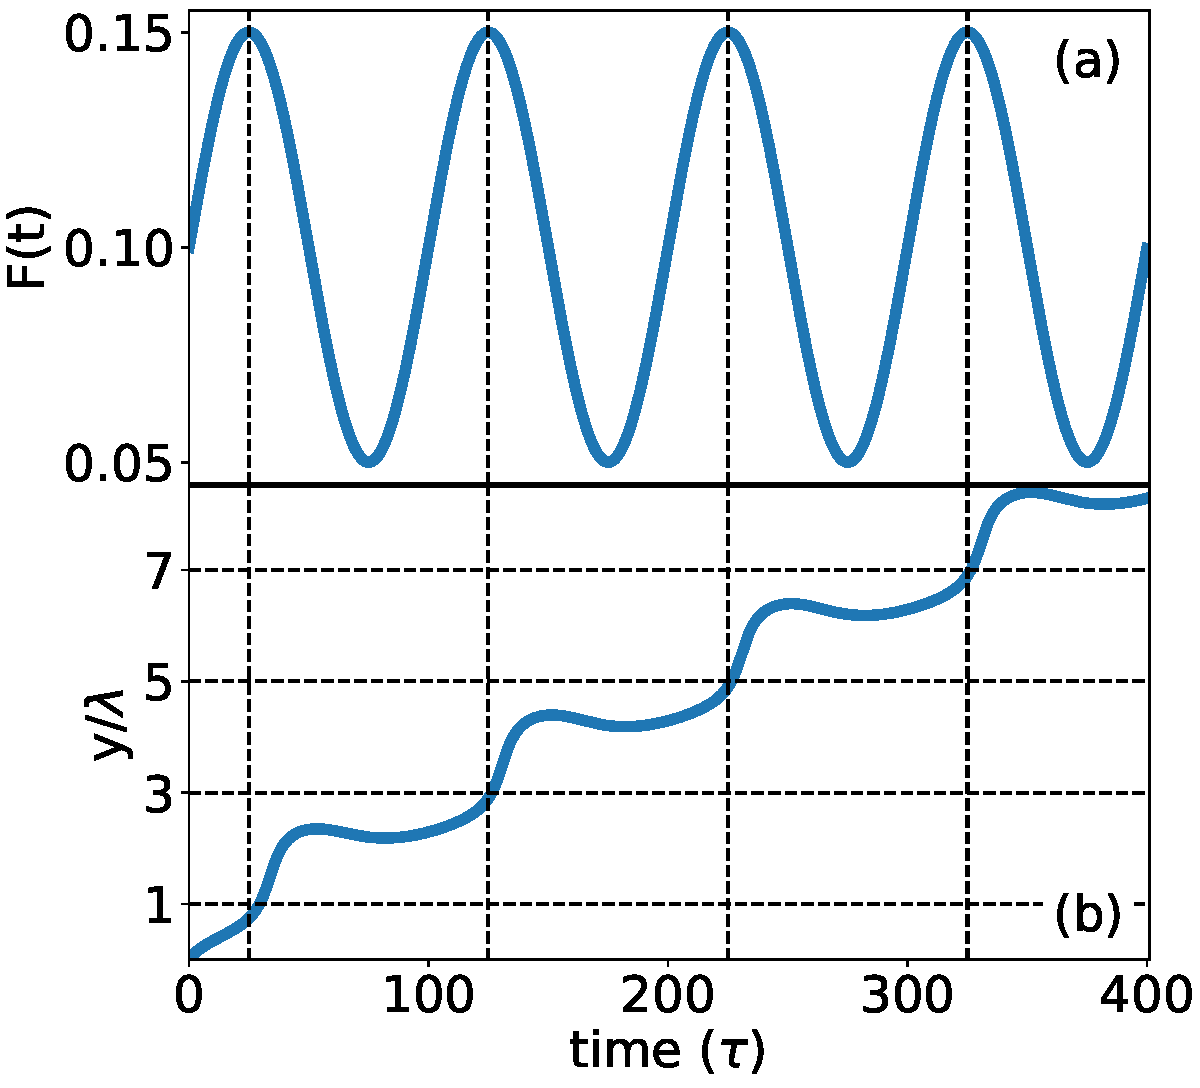
\includegraphics[width=\columnwidth]{single_particle.pdf}
\caption{(a) The applied driving force $F^d(t)$ (orange) in Eq.~\ref{eq:drive}
  where the parameter $F^{dc}$ (blue) is slowly increased from zero
  to a constant value
  as described in the text.  (b) 
  The $y-$position of the driven particle
  as a function of time %of a single driven particle
  normalized by the period of the substrate $\lambda$.
  }
\label{fig:0}
\end{figure}
\end{center}

The competition between the driving force and landscape potential
can produce a variety of hopping patterns in the particle motion.
If $A_p$ is large compared to the extrema of $F^{d}(t)$,
the particle oscillates back and forth
in a single minima
with no net velocity.  
%In Fig.~\ref{fig:0}

%reaching a minimum position
%of $y/\lambda = 1$
%over the total period $T = 100$.
%The average velocity $\bar{v}_y$
%is the average displacement $\Delta y = y(t_0+T) - y(t_0)$
%over the period of the driving force.
%In Fig. ~\ref{fig:0}
%the average displacement during one time period is a single wavelength
%of the substrate $y(t_0+T) - y(t_0) = \lambda$.
%single dc case with figure
%dc_current 0.01
%ac_current 0.05
%ac_frequency 0.01
%fp_y 0.1

The relative values of $F^{ac}$, $F^{dc}$ and $A_p$
control the rate and length of the particle hops
forward and backward in the landscape.
When $F^{dc} - F^{ac} < -A_p$ the particle
moves in the negative y-direction 
during part of the cycle.
We explore this in Ex.~\ref{ex:backwards}.
To explore the possible hopping patterns,
we sweep through a range of $F^{dc}$ for fixed $F^{ac}$ and $A_p$,
as shown in Fig.~\ref{fig:1}(b).
We keep $F^{dc}$ constant
for $\Delta t = 10^4$ timesteps
and 
sample the average velocity $\langle v_y \rangle $ 
as a function of $F^{dc}$.

We perform this sweep for several values
of $F^{ac}$ including the limiting case that the applied force
is a constant value.
When $F^{ac} = 0$, no steps appear
in the $\langle v_y \rangle $ vs $F^{dc}$ curve.  

Synchronization
of the driving force with the landscape,
despite the overall magnitude
of $F^{dc}$.





The particle 
achieves a variety of oscillation modes as a function of $F^{dc}$.
A mode is a periodic pattern of hops
with a constant average particle velocity, $\bar{v}_{y}$
over a range of driving forces $F^{dc}$.
We illustrate mode-locking in 
the velocity-force plot in Fig.~\ref{fig:1}(b).
Here $\langle v_{y} \rangle$ is increasing in non-uniform steps,
with a quantized height of
$\langle v_{y} \rangle = n \lambda f$,
where $n$ is an integer.  
%$\lambda = L/N_p = 36.5/20 = 1.825$ is the spatial period, or wavelength
%of the landscape,
%and $f = 0.01$ cycles per time unit.

Phase locked steps occur for average displacements integer
multiples of the substrate period $n\lambda$.

Our simulations reproduce results presented in 
Juniper {\it et al.} \cite{Juniper2015, Juniper2018}
which demonstrated
mode locking in
experiments and simulations of 
driven colloids on a
optical periodic landscape.

We 
show the dynamics 
in supplementary materials \cite{supp1}.

\begin{center}
\begin{figure}[h!]
\centering
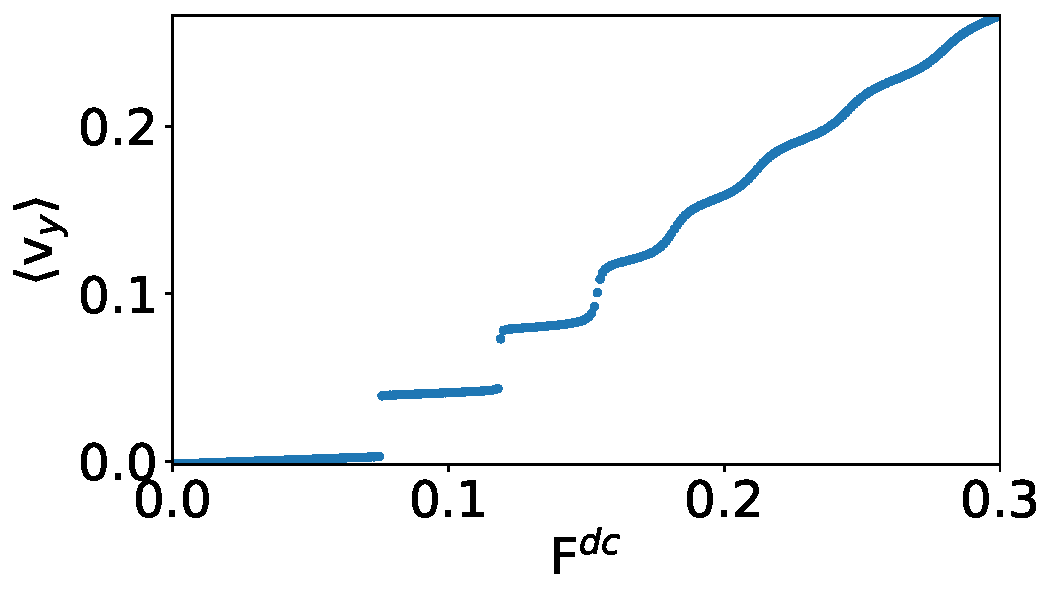
\includegraphics[width=\columnwidth]{sweep_FDC_vs_vx.pdf}
\caption{(Average particle velocity  $\langle v_{y} \rangle$ as a function of $F^{dc}$.  We fix the amplitude of $F^d(t)$ as $F^{ac}=0.05$ as in Fig.~\ref{fig:0}}.
\label{fig:1}
\end{figure}
\end{center}

%In the animation available in Ref.~\cite{supp1} the magenta dot represents the average velocity of the particle $\langle v_{y} \rangle$ at which the particle in Fig. 1(a) is moving.

%We examine
The period of the substrate
can be used to control the
intrinsic velocity of the dc driven particle,
and the applied ac drive can cause mode-locking
which appears as non-linear 
steps in the force-velocity relationship.

Fundamental models
of synchronization 
can include many coupled oscillators
or focus on 
a single particle driven across a periodic potential landscape.
Single particle studies 
are useful to understand synchronization
in the absence of collective effects.
%A single particle particle oscillator
%within a potential well is 
%much like a skateboarder in a half-pipe or
%a child on a swing
%moving back and forth. % through equilibrium.  % \cite{}.
The relationship between the driving force and
landscape can change the pattern of motion.  
With a constant or 
dc drive the landscape modulates 
the particle velocity, below some threshold  
the dc force is not strong enough to push the particle
across a potential maximum so the average velocity is zero,
a phenomena refered to as pinning \cite{Reichhardt2017}.  
%and dissipating energy from the system at all driving forces.
A sinusoidal or ac drive creates mode-locking,
where the average particle velocity
is fixed for a range of dc drive forces \cite{Reichhardt2015}.



\section{Synchronized particle chains}
\label{sec:sync}
The interaction forces between colloids can be controlled 
by altering the chemistry of the suspending fluid
or surface ligands of the particles.
Thus colloids can 
be modified to mimic different
systems such as hard spheres interacting via contact forces \cite{},
dipole interactions \cite{},
and long range electrostatic interactions \cite{}.

Mode-locked 
colloid dynamics have been achieved in 
experiments \cite{Juniper2015, Lutz2004} and
simulations \cite{Herrera-Velarde2007, Herrera-Velarde2008} 
for a variety of interaction types such as 
magnetic dipoles and electric forces.
%-----------------------------------------------------------
%particle interaction types
%Particles which interact over long distances
%include colloids, magnetic beads, superconducting vortices, dusty plasmas, electron gases. [more%e detail and references]
%Particles which interact over short distances include
%bubble arrays/emulsions [more systems and references].----------------------
%The presence of a modulating surface
%can modify these patterns in a variety of ways,
%changing the onset of dynamical flows,
%and the overall flow patterns.
%  adjustable strength, geometry and length scale of substrate potential
%Baumgartl, Brunner, Bechinger, PRL 93, 168301 (2004).
%Baumgartl, Zvyagolskaya, Bechinger, PRL 99, 205503 (2007).

%-----------------------------------------------
%environments
Particles in confined geometries behave differently than free particles.
Stabilized charged particles form patterns
due to the interplay of the confining landscape 
and particle interactions.
Narrow channels studies are useful to provide insights 
of how particles move through systems 
such as charge carries in quantum wires \cite{Tarucha1995} and
slime molds in microchannels \cite{Gholami2015}.
%Biological systems such as
%neuron axons and capillaries can also be studied
%with these models [more detail and references].
%Many such systems execute local oscillations
%about stable points [elaborate].
%------------------------------------
 In multi-particle simulations, we confine
 the particles to a narrow region
 along the $x-$direction 
 using a periodic function 
 \begin{equation}
   U_{q1D}(x) = U_{q0} \cos{(\pi x / L)}
     \label{eq:xsubstrate}
 \end{equation}
 where $U_{q0}$ defines the channel depth.
 %%We could also use a Gaussian function.
 This 
 quasi-one-dimensional geometry
 confines the particles
 primarily to move 
 along the y-direction
 but allows for some lateral motion of particles.
 Otherwise the repulsive interaction between
 particles would cause them to spread throughout the system.
 %
 The total landscape potential energy function is the sum
 \begin{equation}
   U_{landscape}(x,y) =  U_{q1D}(x) + U_{washboard}(y)
   \label{eq:xylandscape}
 \end{equation}

We explore collective effects in a 
twenty particle system confined to a narrow channel, as shown in Fig. 2a).  We create the confining channel with a sinusoidal function
with a single period.
\begin{equation}
  \label{eq:channel}
  U_l(x) = U_{0x} \cos{(\pi x/L)}.
\end{equation}
%where the trough heights is larger  $V_{0x}$,
%and the associated force
%\begin{equation}
%\vec{F}=-\nabla V(x) = -\frac{dV}{dx} \hat{x} = - \frac{V_{0x} \pi}{L} \sin{(\pi x/L)} \hat{x}
%\end{equation}
%restores particles to the center of a long narrow region of the simulation.
The landscape potential energy is illustrated in Fig.~\ref{fig:2}(a)
where red regions are high potential
and blue regions are low potential.

 We model particle interaction forces
$\vec{F}_{ij} = -\nabla U_{ij}(r_{ij})$ 
with
the Yukawa potential $V_{ij} = U_{ij} / q$ 
\begin{equation}
  V_{ij}(r_{ij}) = \frac{E_0}{r_{ij}} e^{-\kappa r_{ij}},
  \label{eq:yukawa}
\end{equation}
where particle $i$ and $j$ are distance
$r_{ij} = |\vec{r}_i - \vec{r}_j|$ apart.
This 
screened Coulomb potential
%$E_0=2$ scales strength of repulsion
is scaled in terms of energy unit $E_0$
defined in Table ~\ref{tab:1}.
[elaborate for students $F_{Coulomb} = = k q_1 q_2 / r^2$, check scaling/units].
$\kappa = 1/R_0$ is the screening parameter 
that describes the length scale at
which particles interact.
We fix the screening length scale $R_0$ to be $a_0$
(i.e. unity in simulation units).
In experiments charge screening is observed
due to ions in the suspending fluid and
the charges of surrounding particles
which
reduces the interaction range of individual particles. % \cite{}.
Because the particles interact over short ranges, 
the numerical models can be run efficiency
using a neighbor list algorithm
determined using a cell method.
[explain and reference!]

Newton's second law can be rearranged %for the velocity
to
the equation of motion a single particle subject to collective effects is 
\begin{equation}
  \eta \vec{v}_i = \vec{F}^l_{i} + \sum_{i \neq j}^{N} \vec{F}_{ij} + \vec{F}_{D}(t).
    \label{eq:motion}
\end{equation}

The initial configuration of the system is shown in 
Fig.~\ref{fig:2}(a).  
We annealed the system into a ground-state configuration
by raising the system to a high temperature $T$,
and slowly lowering the temperature in steps of $dT=-0.01$
until the particles form a buckled chain in the low region of the channel
due to the
competition between particle repulsion and channel confinement.
The interparticle forces between neighboring particles
cause the system to form a buckled chain. % when the system is annealed.
The molecular dynamics of simulated annealing
is described in Ref.~\ref{Allen2017}.
Once the ground state particle configuration is obtained,
no further annealing is necessary,
so the
our simulations begin with particle configurations
that result from the annealing process,
as listed in Appendix [ref] and available in supplementary material.

When a single particle is driven, the neighboring particles act similarly to a periodic landscape to impede its motion. A driven particle can exhibit mode locking with a well-chosen ac drive and frequency. In the attached movie, Figure2.mp4, we show the complex dynamics of mode locking, where the driven particle leap-frogs past the other particles. 

\begin{center}
\begin{figure}[h!]
\centering
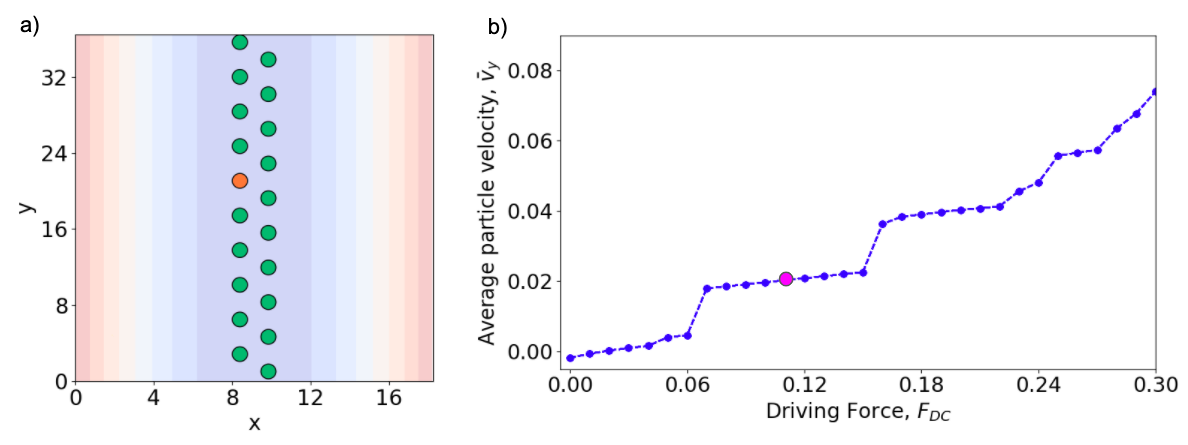
\includegraphics[width=\columnwidth]{twenty}
\caption{\textbf{(a)} A single particle (colored orange - mark in some manner for non-color views) is driven with a constant amplitude $F^{ac}$ and frequency $\omega$ through 19 neighboring particles (colored green - mark differently) confined by a quasi one-dimensional channel. The landscape is colored as in Fig.~\ref{fig1}(a). \textbf{(b)} Average $\bar{v}_{y}$ versus $F^{dc}$, where $\bar{v}_{y}$ is the average particle velocity of the driven particle in the y-direction.}
\label{fig:2}
\end{figure}
\end{center}

\section{Kinked system}
\label{sec:kink}	% You can label sections for reference
We confine $N$ particles to $N-1$ troughs to create a
local high density region.
$F^{dc}/F^{ac} = 1$ [CHECK!]



%\section{Quasi-periodic substrate}
%\label{sec:quasiperiod}	% You can label sections for reference

%\section{Chaotic dynamics}
%\label{sec:chaos}	% You can label sections for reference

\section{Associated problems}
\label{sec:problems}	% You can label sections for reference

\begin{enumerate}
\item Stokes' law describes the viscous drag on a sphere
  moving at velocity $\vec{v}$ as 
  $\vec{F}^{lin} = 3 \pi \eta D \vec{v}$ \cite{}
  where $\eta$ is the dynamic fluid viscosity and 
  $D$ is the particle diameter.
  (In simulation we
  subsume the constants $3 \pi D$
  such that $\eta \rightarrow 3 \pi D \eta$.)
  Often drag forces are
  modeled as a polynomial series
  $\vec{F}^{drag} = \vec{F}^{lin} + \vec{F}^{quad} + ... $.
  Truncating the series to the first term
  is justified by calculating the Reynolds number  
  $R = D v \rho / \eta$
  where $\rho$ is the fluid density and $v$ the particle's speed.
  When $R$ is small, the quadratic and higher order drag terms
  may be ignored in favor of the linear drag term.

  Demonstrate the Reynolds number is low
  for this system.
  
  Reasonable experimental values for
  a colloid are $D = 1 \mu m$ and $v \sim 1 \mu m /s$.
  Viscosity of water decreases with temperature
  from $1.3 \times 10^{-3} Pa-s$ at $10^{\circ}C$ to 
  from $0.31 \times 10^{-3} Pa-s$ at $90^{\circ}C$,
  making $\eta \sim 10^{-3} Pa-s$,
  where 1 pascal $ = 1 Pa = 1 N/m^2$.
  Likewise the density $\rho$ varies with temperature
  and $\rho \sim 10^3 kg/cm^3$ is a reasonable approximation.
  
  [citation for these values better than wikipedia] \cite{} %CONFIRM!
  %density $\rho = 0.9982 g/cm^3$
  %https://ascelibrary.org/doi/pdf/10.1061/9780784408230.ap02

This model should be familiar to readers
of a standard classical mechanics text, such as Ref.~\cite{Taylor2005}
when studying 
models Millikan's oil drops.

[could certainly do more with this question to make it more computational.  For instance, plot $R$ as a function of any of the parameters $v$, $D$ and $\rho$, include a temperature dependent $\eta(T)$ in the Brownian system.  Suggest students model something big and include inertia and quadratic drag, but then we're fairly off topic...]

\label{ex:reynolds}

\item Newton's second law states that
  the acceleration of a particle $i$
  is proportional to 
  the sum of forces on a particle 
  \begin{equation}
  m_i \vec{a}_i = \sum \vec{F}_i
  \label{eq:n2l}
  \end{equation}
  where the constant of proportionality is the
  inertial mass $m_i$
  The addition of a dissipative force in a dynamical model
  on a colloid is typically modeled
  with a drag force proportional to the particle's velocity
  in the opposite direction of motion 
  $\vec{F}^{drag} = - \eta \vec{v}_i$
  where $\eta$ is the drag coefficient.
  Demonstrate
  the ratio of $m/\eta$ has units of time, 
  %This ratio of the acceleration coefficient $m$
  %to the drag coefficient $\eta$
  %is
  known as the momentum relaxation time.
  The momentum relaxation time is 
  known to be small for
  particles with low Reynolds numbers,
  indivating 
  a regime in which the acceleration term can be ignored
  entirely.
  Demonstrate that a particle confined to a landscape exerting force
  $F^l(\vec{r}_i)$ subject to a time dependent drive $F^d(t)$
  can be modeled with the equation of motion described in 
  Eq.~\ref{eq:motion}. 
  \label{ex:n2l}

\item
  Generally when solving differential equations,
  the Euler method is effective for solving linear equations,
  such as the one-dimensional 
  $f(y) = df/dy$ 
  but not higher order methods.

  The Verlet method simplifies to

  %FOLLOW UP WITH THIS!
  Because we are performing molecular dynamics
  for a single particle on a smooth potential energy landscape,
  we use a large simulation time step of 
  $\Delta t = 0.01$.
  In Sec.~\ref{sec:sync},
  we decrease the time step
  to treat multiple particle interactions.

  \label{ex:euler}

\item Drawing the contour

  The code for generating
a two dimensional colored plot
of the potential landscape
is calculated by evaluating
the analytic function in Eq.~\ref{eq:landscape}
for a grid of values $(x_n,y_n)$.
%is included in the supplementary material,
  
\item Kuramoto model = overdamped interacting rotors/oscillators are used to model coupled oscillator systems - no substrate or external drive so far as I can see - this seems baked into the oscillator properties/interactions
%D. Métivier, L. Wetzel, and S. Gupta
%Onset of synchronization in networks of second-order Kuramoto oscillators with delayed coupling: Exact results and application to phase-locked loops
%PHYSICAL REVIEW RESEARCH 2, 023183 (2020)

\item {\bf Brownian motion}
  is a temperature and viscosity dependent
  phenomena. \cite{}
  Consider the consequences of a non-zero temperature on the simulation, in which particles will collide with invisible particles making up the suspending fluid.  These collisions are more likely at higher temperature due to the increased kinetic energy of the fluid particles, as described by the Maxwell-Boltzmann distribution \cite{}.  In molecular dynamics simulations temperature effects can be modeled by including randomized forces $f^T$ to emulate the motion of particles undergoing Brownian motion.  A distribution of randomizes forces contributes equally in all directions such that the force averaged over a finite time interval is zero $\langle f^T(t) \rangle = 0$.  Random distributions of contain no correlations over the independent variable (time in this case) $\langle f^T(t) f^T(\tau)\rangle = 2 \eta k_B T \delta(t-\tau)$ where the energy $k_B T$ derived from the Boltzmann constant $k_B$ and temperature $T$ has energy units $E_0$.  \cite{Allen2017}

  With no applied driving force, measure the minimum temperature required for a single particle to hop between minima in the potential landscape.

  Measure the rate of diffusion.

\item Frenkel-Kontorova and competing length scales for low temperature systems where thermal fluctuations are negligible

  \item The Fokker-Planck Equation

  \item Aubrey-Kontorova + commensurability

  \item nanotribology

    kink motion
    Vanossi et al J.Phys.: Condens. Matter 19 (2007)


    
\end{enumerate}

\section{Conclusion}
\label{sec:conclusion}	% You can label sections for reference
Due to the relative ease of
manipulation and imagining, 
colloids are used as experimental models
for systems relatively hard to access and visualize. 
%SAME SENTENCE TWICE
Collections of colloids can
be used to study the properties of solids and liquids
%comprised of smaller particles
%such as atoms \cite{} or electrons \cite{}
or more exotic systems 
such as cold atoms or electron gases \cite{Grier2003}.

%Oscillators ordered into chains or lattices.
%has many important
%technological applications
Dynamical mode-locking
is %often
observed
in quantum electronic
devices such as Josephson junctions \cite{Josephson1962,Josephson1965}.
A single junction contains 
two superconductoring layers which sandwich an insulating layer.
When subject to an external voltage,
Cooper pairs in the superconducting materials
tunnel through the insulating layer.
Phase-locking is observed as 
%phase-locked current loops \cite{} 
stepped regions in current-voltage (I-V) relationship in these devices,
where voltage is the analog of external driving force
and current is that of particle velocity.
%where a constant current results from a range of voltages
%due to the quantized nature of the tunneling probability [NOT QUITE RIGHT...].
%instead of ohmic relationships.
Known as Shapiro steps, % \cite{},
these phase locked currents  
have been observed due to applied ac voltages in 
single Josephson junctions \cite{Shapiro1963, Golubov2004} and
coupled arrays of junctions \cite{Benz1990}.
%either in 
%velocity-force curves and voltage-current curves \cite{Golubov2004}.
Shapiro steps vary in width depending on the strength of the
applied ac forces,
and are observed in a variety of systems
displaying
%are hallmarks of
non-Ohmic behavior in voltage-current curves,
including
ac and dc driven
charge and spin density waves.

%where these steps are generated
%by the tendency of the response of a system
%to be flat across a range of applied driving forces or voltages,
%which can be probed with
%  atoms on surfaces.
%  voltage driven superconducting vortices
%  confined in a Josephson junction,

%
%
%mini review of synchronization in electronics
%careful - the following is all simulations
%Recent studies demonstrate
%that coupled electronic oscillators can be
%programmed for use as micro-controllers for robotic locomotion \cite{Dutta2019}.


%%%%%%%%%%%%%%%%%%%%%%%%%%%%%%%%%%%%%%%%%%%%%%%%%%%%%%%%%%%%%%%%%%
\section{Supplementary Materials}



\begin{acknowledgments}

  We acknowledge Harvey Gould and Jan Tobochnik,
  who invited us to write the article and
  supported its development.
  Charles and Cynthia Reichhardt advised 
  the project and provided the original molecular dynamics code
  written in the C programming language.
  We acknowledge funding from the M.J. Murdock Charitable Trust
  and the Pacific Research Institute for Science and Mathematics (PRISM).

\end{acknowledgments}


\begin{thebibliography}{99}
% The numeral (here 99) in curly braces is nominally the number of entries in
% the bibliography. It's supposed to affect the amount of space around the
% numerical labels, so only the number of digits should matter--and even that
  % seems to make no discernible difference.

  %useful quick ref
  %http://www.scholarpedia.org/article/Synchronization
  
  %intro to oscillators
\bibitem{Pikovsky2003} A. Pikovsky, M. Rosenblum, and J. Kurths, {\it Synchronization: A Universal Concept in Nonlinear Sciences} (Cambridge Univ. Press, Cambridge, 2003).
  
\bibitem{Bennett2002} M. Bennett, M.F. Schatz, H. Rockwood, and K. Wiesenfeld, Huygens' clocks, Proc. Roy. Soc. A {\bf 458}, 563 (2002).
  
\bibitem{Okamoto2016} K. Okamoto, A. Kijima, Y. Umeno, and H. Shima. Synchronization in flickering of three-coupled candle flames. Sci Rep {\bf 6}, 36145 (2016)

\bibitem{Arane2009} T. Arane, A. K. R. Musalem and M. Fridman, Coupling between two singing wineglasses, Am. J. Phys. {\bf 77}, 1066 (2009). %; https://doi.org/10.1119/1.3119175
  
\bibitem{Jia2015}  J. Jia, Z. Song, W. Liu, J. Kurths, and Xiao, J. Experimental study of the triplet synchronization of coupled nonidentical mechanical metronomes. Sci. Rep. {\bf 5}, 17008 (2015).

%Synchronization of a thermoacoustic oscillator by an external sound source
%G. Penelet and T. Biwa
%American Journal of Physics 81, 290 (2013); https://doi.org/10.1119/1.4776189
  
  %biological examples
  
\bibitem{Portugal2014} S. Portugal, T. Hubel, J. Fritz, S. Heese, D. Trobe, B. Voelkl, S. Hailes, A. M. Wilson and J. R. Usherwood.  Upwash exploitation and downwash avoidance by flap phasing in ibis formation flight. Nature {\bf 505}, 399 (2014).

  \bibitem{Aihara2014} I. Aihara, T. Mizumoto, T. Otsuka, H. Awano, K. Nagira, H. G. Okuno and K. Aihara. Spatio-Temporal Dynamics in Collective Frog Choruses Examined by Mathematical Modeling and Field Observations. Sci Rep {\bf 4}, 3891 (2014). 

  \bibitem{Tranchant2016} P. Tranchant, D. T. Vuvan, and I. Peretz, Keeping the Beat: A Large Sample Study of Bouncing and Clapping to Music. PLoS ONE 11(7): e0160178. (2016).

  \bibitem{MartinHall1999} G. Martin Hall, Sonya Bahar, and Daniel J. Gauthier, Prevalence of Rate-Dependent Behaviors in Cardiac Muscle. Phys. Rev. Lett. {\bf 82}, 2995 (1999).

  \bibitem{Singer1999} W. Singer. Striving for coherence. Nature, {\bf 397} 391, 1999.

    %technological applications
    \bibitem{Dutta2019} Dutta, S., Parihar, A., Khanna, A. et al. Programmable coupled oscillators for synchronized locomotion. Nat Commun {\bf 10}, 3299 (2019).
    
    %condensed matter intro
    \bibitem{Bak1986} P. Bak. The Devil's Staircase. Physics Today {\bf 39}, 12, 38 (1986).

    \bibitem{Lissajous1857} J. A. Lissajous.  "Mémoire sur l'Etude optique des mouvements vibratoires,"  Annales de chimie et de physique, 3rd series, 51 (1857) 147-232

    \bibitem{Tong1997} E. Y. C. Tong, Lissajous figures, The Physics Teacher {\bf 35}, 491 (1997).

    \bibitem{Purcell1977} E. M. Purcell, Life at low Reynolds numbers, Am. J. Phys. {\bf 45}, 3–11 (1977).

      %PRACTICAL APPLICATION
    %\bibitem{Agrawal2013} D. K. Agrawal, J. Woodhouse, and A. A. Seshia, Observation of locked phase dynamics and enhanced frequency stability in synchronized micromechanical oscillators, Physical Review Letters {\bf 111}, 084101 (2013).

    \bibitem{Josephson1962} B. D. Josephson, Phys. Letters {\bf 16}, 25 (1962). 
    \bibitem{Josephson1965} B. D. Josephson, Advan. Phys. {\bf 14}, 419 (1965).

    \bibitem{Stewart1968}  W. C. Stewart CURRENT‐VOLTAGE CHARACTERISTICS OF JOSEPHSON JUNCTIONS Appl. Phys. Lett. 12, 277 (1968).
      
    \bibitem{Shapiro1963} S. Shapiro, Josephson currents in superconducting tunneling: the effect of microwaves and other observations, Phys. Rev. Lett. 11, 80 (1963).

    \bibitem{Benz1990}  S. P. Benz, M. S. Rzchowski, M. Tinkham, and C. J. Lobb, Fractional giant Shapiro steps and spatially correlated phase motion in 2D Josephson arrays, Phys. Rev. Lett. 64, 693 (1990); D. Dom´ınguez and J. V. Jos´e, Giant Shapiro steps with screening currents, Phys. Rev. Lett. 69,
514 (1992).

    \bibitem{Golubov2004} A. A. Golubov, M. Yu. Kupriyanov, and E. Il’ichev. The current-phase relation in Josephson junctions, Rev. Mod. Phys. {\bf 76}, 411 (2004).

      quote: Phase engineering techniques are used to control the dynamics of long-bosonic Josephson-junction arrays built by linearly coupling Bose-Einstein condensates.
    \bibitem{Zhang2020} Dengling Zhang, Haibo Qiu, and Antonio Muñoz Mateo, Unlocked-relative-phase states in arrays of Bose-Einstein condensates, Phys. Rev. A {\bf 101}, 063623 (2020).

      %reichhardt review
    \bibitem{Reichhardt2017} C. Reichhardt and C. J. Olson Reichhardt, “Depinning and nonequilibrium dynamic phases of particle assemblies driven over random and ordered substrates: a review,” Rep. Prog. Phys. 80, 026501 (2017).

    \bibitem{Reichhardt2015} C. Reichhardt, and C. J. O. Reichhardt,  Shapiro steps for skyrmion motion on a washboard potential with longitudinal and transverse ac drives. Phys. Rev. B {\bf 92}, (22). (2015).
      
    \bibitem{Juniper2015} M. P. N. Juniper, A. V. Straube, R. Besseling, D. G. A. L. Aarts, and R. P. A. Dullens, Microscopic dynamics of synchronization in driven colloids. Nat. Commun. 6, 7187 (2015).

    \bibitem{Juniper2018} Juniper, M. P. N., Zimmermann, U., Straube, A. V., Besseling, R., Aarts, D. G. A. L., Löwen, H., and Dullens, R. P. A.  Dynamic mode locking in a driven colloidal system: Experiments and theory. New Journal of Physics, 19(1). (2017).  %https://doi.org/10.1088/1367-2630/aa53cd
      
    \bibitem{Herrera-Velarde2008} S. Herrera-Velarde and R. Castañeda-Priego, Superparamagnetic colloids confined in narrow corrugated substrates, Phys. Rev. E {\bf 77}, 041407 (2008).

    \bibitem{Herrera-Velarde2007} S. Herrera-Velarde and R. Castañeda-Priego, J. Phys.: Condens. Matter 19, 226215 (2007).

    \bibitem{Grier2003} D. G. Grier, A revolution in optical manipulation. Nature {\bf 424}, 810 (2003).

     \bibitem{Ashkin1997} Arthur Ashkin, Optical trapping and manipulation of neutral particles using lasers, Proc. Natl. Acad. Sci. U.S.A. 94, 4853–4860 (1997).
        
      \bibitem{Volpe2013} G. Volpe and G. Volpe, Simulation of a Brownian particle in an optical trap, Am. J. Phys. 81 (3), March 2013
        
%Lutz  created 1D circular channels by means of scanning optical tweezers in order to avoid the presence of lateral confinement walls
    \bibitem{Lutz2004} C. Lutz, M. Kollmann, and C. Bechinger, Phys. Rev. Lett. {\bf 93}, 026001 (2004); C. Lutz, M. Kollmann, C. Bechinger, and P. Leiderer, J. Phys.: Condens. Matter {\bf 16}, S4075 (2004).

    \bibitem{Tarucha1995}  S. Tarucha, T. Honda,  T. Saku, Solid State Commun. 1995, 94, 413.

    \bibitem{Gholami2015} A. Gholami, O. Steinbock, V. Zykov, and E. Bodenschatz, Flow-Driven Waves and Phase-Locked Self-Organization in Quasi-One-Dimensional Colonies of Dictyostelium discoideum, Phys. Rev. Lett. {\bf 114}, 018103 (2015).

      %Molecular dynamics references

    \bibitem{Frenkel2001} D. Frenkel and B. Smit, Understanding Molecular Simulation: From Algorithms to Applications (Academic Press, London, 2001).
      
    \bibitem{Allen2017} M. P. Allen and D. J. Tildesley, Computer Simulation of Liquids.  Second Edition. Oxford University Press (2017).

    \bibitem{Taylor2005} J. Taylor,  Classical mechanics. University Science Books (2005).
      
\bibitem{supp1} See Figure1.mp4 in appropriate %\url{}

%\bibitem{latexsite} \LaTeX\ Project Web Site, \url{<http://www.latex-project.org/>}.

%\bibitem{wikibook} \textit{\LaTeX} (Wikibook), \url{<http://en.wikibooks.org/wiki/LaTeX/>}.

%\bibitem{latexbook}Helmut Kopka and Patrick W. Daly, \textit{A Guide to
%\LaTeX}, 4th edition (Addison-Wesley, Boston, 2004).

%\bibitem{revtex} REV\TeX\ 4 Home Page, \url{<https://authors.aps.org/revtex4/>}.

%\bibitem{cloudLaTeX} On the other hand, you can avoid the installation process
%entirely by using a cloud-based \LaTeX\ processor such as ShareLaTeX,
%\url{<https://www.sharelatex.com/>}, or write\LaTeX, \url{<https://www.writelatex.com/>}.

%\bibitem{nevermindlogic} In typography, aesthetics often takes precedence over logic.

%\bibitem{FontEncodingComment} Please don't try to handle foreign characters 
%and accents with the \texttt{inputenc} and \texttt{fontenc} packages, which 
%are incompatible with AJP's editing process.

%\bibitem{wikimathpage} See the Mathematics chapter of Ref.~\onlinecite{wikibook} for an excellent overview of math symbols and equations, with examples.

%\bibitem{labelnames} Thinking up a good label name takes a moment, but 
%it's worth the trouble; we strongly advise against using labels like 
%\texttt{eq2}, which become extremely confusing after you decide to add 
%another equation before Eq.~(\ref{deriv}).

%\bibitem{footnotes} You need to process a file twice to get the counters correct.

%\bibitem{mermin} N. David Mermin, ``What's wrong with these equations?,'' 
%Phys. Today \textbf{42} (10), 9--11 (1989).  
% Note that the issue number (10) in this citation is required, because
% each issue of Physics Today starts over with page 1.  Also note the use of
% an en-dash (--), not a hyphen (-), for the page range.

%\bibitem{editorsite} American Journal of Physics Editor's Web Site, 
%\url{<http://ajp.dickinson.edu>}.

%\bibitem{feynman} Richard P. Feynman, Robert B. Leighton, and Matthew Sands, 
%\textit{The Feynman Lectures on Physics, Vol.\ 1} (Addison-Wesley, 1964), p.~3-10.
% Note that this book is paginated by chapter; "3-10" is a single page reference
% that uses a hyphen, not a range of pages that would us an en-dash (--).

%\bibitem{noBIBTeX} Many \LaTeX\ users manage their bibliographic data with 
%a tool called BIB\TeX.  Unfortunately, AJP cannot accept BIB\TeX\ files; all 
%bibliographic references must be incorporated into the manuscript file
%as shown here, at least when you send an editable file for production.

%\bibitem{dyson} Freeman J. Dyson, ``Feynman's proof of the Maxwell equations,''
%Am. J. Phys. \textbf{58} (3), 209--211.  
% The issue number (3) in this citation is optional, because AJP's pagination 
% is by volume.

%\bibitem{examplevolume} M. R. Flannery, ``Elastic scattering,'' in 
%\textit{Atomic, Molecular, and Optical Physics Handbook}, edited by
%G. W. F. Drake (AIP Press, New York, 1996), p.~520.

%\bibitem{AIPstylemanual} \textit{AIP Style Manual}, 4th edition (American 
%Institute of Physics, New York, 1990). Available online at 
%\url{<http://www.aip.org/pubservs/style/4thed/toc.html>}. Although parts of 
%it have been made out of date by advancing technology, most of this manual 
%is still as useful as ever. Just be sure to follow AJP's specific rules
%whenever they conflict with those in the manual.

\end{thebibliography}

% If your manuscript is conditionally accepted, the editors will ask you to
% submit your editable LaTeX source file.  Before doing so, you should move
% all tables and figure captions to the end, as shown below.  Tables come 
% first, followed by figure captions (with figure inclusions commented-out).
% Figures should be submitted as separate files, collected with the
% LaTeX file into a single .zip archive.

%\newpage   % Start a new page for tables

%\begin{table}[h!]
%\centering
%\caption{Elementary bosons}
%\begin{ruledtabular}
%\begin{tabular}{l c c c c p{5cm}}
%Name & Symbol & Mass (GeV/$c^2$) & Spin & Discovered & Interacts with \\
%\hline
%Photon & $\gamma$ & \ \ 0 & 1 & 1905 & Electrically charged particles \\
%Gluons & $g$ & \ \ 0 & 1 & 1978 & Strongly interacting particles (quarks and gluons) \\
%Weak charged bosons & $W^\pm$ & \ 82 & 1 & 1983 & Quarks, leptons, $W^\pm$, $Z^0$, $\gamma$ \\
%Weak neutral boson & $Z^0$ & \ 91 & 1 & 1983 & Quarks, leptons, $W^\pm$, $Z^0$ \\
%Higgs boson & $H$ & 126 & 0 & 2012 & Massive particles (according to theory) \\
%\end{tabular}
%\end{ruledtabular}
%\label{bosons}
%\end{table}

%\newpage   % Start a new page for figure captions

%\section*{Figure captions}

%\begin{figure}[h!]
%\centering
%\includegraphics{GasBulbData.eps}   % This line stays commented-out
%\caption{Pressure as a function of temperature for a fixed volume of air.  
%The three data sets are for three different amounts of air in the container. 
%For an ideal gas, the pressure would go to zero at $-273^\circ$C.  (Notice
%that this is a vector graphic, so it can be viewed at any scale without
%seeing pixels.)}

%\label{gasbulbdata}
%\end{figure}
      
\end{document}


%%%%%%%%%%%%%%%%%%%%%%%%%%%%%%%%%%%%%%%%%%%%%%%%%%%%%%%%%%%%%%%%%%
\section{Supplementary Materials}

\subsection{Gridded Contour Plot of landscape}
%code is located in
%~/pymodules/animation_code/channel_colloid_movie_maker.py

\begin{verbatim}
##########################################################
#ADD CONTOUR PLOT
##########################################################
def add_contour(ax,L,N,corrugated = True):
    '''
    Hardwired to color in the quasi1D potential to contain 
    the particles in a trough.  
    Can also add the washboard/corrugated substrate.

    Required Arguments

    Optional Arguments:

    corrugated (default = True)  
    Adds the washboard in the y-direction.  
    Hardwired for a single parameter set.    
    '''

    a_p = L/N

    #assuming Tiare's trough system, so we won't want to cover the entire range
    X = np.arange(0, L/2.0, 0.1)
    Y = np.arange(0, L, 0.1)
    X, Y = np.meshgrid(X, Y)

    Z_mag = 2.0 # set by what "looks good"
    Z = Z_mag*np.sin(2*np.pi*X/L)
    if corrugated == True:
        Z += np.sin(2*np.pi*(Y+1.75)/a_p) 

    cmap=cm.coolwarm_r

    #alphs is the degree of transparency, again, set by what looks good.
    cset = ax.contourf(X, Y, Z, cmap=cmap,alpha=0.25)

    #ax1.set_xlim(15,20)
    #ax1.set_ylim(15,20)

    #ax1.set_xlabel(r"$X$")
    #ax1.set_ylabel(r"$y$",rotation='horizontal',ha='right')

    #ax1.set_xticks([])
    #ax1.set_yticks([])
    return
\end{verbatim}

%another confinement technique:
%Acoustic tweezers and surface acoustic wave (SAW) \cite{}
%confines single cells and particles with lower energy than light / lasers
%%X. Ding, J. Shi, S.-C. S. Lin, S. Yazdi, B. Kiraly and T. J. Huang, “Tunable patterning of microparticles and cells using standing surface acoustic waves” Lab Chip, 2012, 12, 2491– 2497.
%%%Acousto-optically generated potential energy landscapes: Potential mapping using colloids under flow Michael P. N. Juniper,1,∗ Rut Besseling,2 Dirk G. A. L. Aarts,1 and Roel P. A. Dullens1


%%%%%%%%%%%%%%%%%%%%%%%%%%%%%%%%%%%%%%%%%%%%%%%%%%%%%%%%%%%%%%%%%%%%%%%%%%%
\subsection{Grid Contour Plot of landscape}
%code is located in
%~/pymodules/animation_code/channel_colloid_movie_maker.py
Testing section - how will putting the code directly in the appendix appear?

\begin{verbatim}
############################################
#ADD CONTOUR PLOT
############################################
def add_contour(ax,L,N,corrugated = True):
    '''
    Hardwired to color quasi1D potential
    that contains 
    the particles in a trough.  
    Can add the washboard/corrugated substrate.

    Required Arguments

    Optional Arguments:

    corrugated (default = True)  
    Adds the washboard in the y-direction.  
    Hardwired for a single parameter set.    
    '''

    a_p = L/N

    #we don't want to cover the entire range
    X = np.arange(0, L/2.0, 0.1)
    Y = np.arange(0, L, 0.1)
    X, Y = np.meshgrid(X, Y)

    Z_mag = 2.0 # set by what "looks good"
    Z = Z_mag*np.sin(2*np.pi*X/L)
    if corrugated == True:
        Z += np.sin(2*np.pi*(Y+1.75)/a_p) 

    cmap=cm.coolwarm_r

    #alpha = transparency. set by what looks good.
    cset = ax.contourf(X,Y,Z,cmap=cmap,alpha=0.25)

    #ax1.set_xlim(15,20)
    #ax1.set_ylim(15,20)

    #ax1.set_xlabel(r"$X$")
    #ax1.set_ylabel(r"$y$",rotation='horizontal',ha='right')

    #ax1.set_xticks([])
    #ax1.set_yticks([])
    return
\end{verbatim}
